\chapter{Rätselseite}

\raggedcolumns
\begin{multicols}{2}
	\section*{Mini-Sudoku}
	Trage in jede Zeile und Spalte die Ziffern 1, 2, 3,~4 so ein, dass A~waagrecht, A~senkrecht, B~senkrecht und F~senkrecht Primzahlen sind!

	\begin{center}
		\begin{tabular}{ |p{0.8cm}|p{0.8cm}|p{0.8cm}|p{0.8cm}| }
		\hline
		  a & b & c & d \\[0.8cm]
		\hline
		  e &   &   &   \\[0.8cm]
		\hline
		  f &   &   &   \\[0.8cm]
		\hline
		  g &   &   &   \\[0.8cm]
		\hline
		\end{tabular}
	\end{center}

	\section*{Gleichung}
	Löse folgende Gleichung, wobei jeder Buchstabe für eine andere Ziffer steht.
	\[\frac{\textrm{EVE}}{\textrm{D\,I\,D}} = \textrm{0,TALKTALKTALK}\dots\]

	\columnbreak
	\section*{Visitenkarten}
	Welchen Beruf haben diese Personen?

	\centerline{Hanne Rubbich \textendash{} Ilztal\\[0.2cm]}
	\centerline{Richie Hersvogt \textendash{} Zell\\[0.2cm]}
	\centerline{Meike Schmettelin \textendash{} Berlin\\[0.2cm]}

	\section*{Kreuzzahlenrätsel}
	Jede Summe, und jeder Summand innerhalb der Summe, darf nur einmal auftreten.

	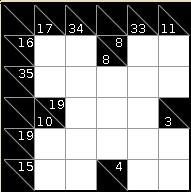
\includegraphics[width=0.9\linewidth]{2011-10-02-134837_191x192_scrot.png}

	\end{multicols}
	\newpage
	\begin{multicols}{2}

	\section*{Minesweeper}
	Ein Spiel was wohl keiner Erklärung mehr bedarf. Jedes Level ist eindeutig lösbar.

	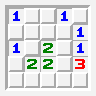
\includegraphics[width=0.45\linewidth]{minepuzzle_gen02tr.png}
	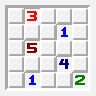
\includegraphics[width=0.45\linewidth]{minepuzzle_gen14tr.png}

	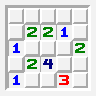
\includegraphics[width=0.45\linewidth]{minepuzzle_gen18tr.png}
	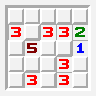
\includegraphics[width=0.45\linewidth]{minepuzzle_gen21tr.png}

	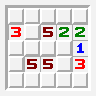
\includegraphics[width=0.45\linewidth]{minepuzzle_gen29tr.png}
	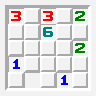
\includegraphics[width=0.45\linewidth]{minepuzzle_gen19tr.png}

	\columnbreak
	\section*{Shikaku}

	Teile das Gitter in Rechtecke, sodass jedes Rechteck genau eine Nummer beinhaltet.
	Die Nummer gibt die Anzahl der Felder an, die das jeweilige Rechteck beinhaltet.

	\arrayrulecolor{black!20} % Linienfarbe
	\renewcommand{\arraystretch}{1.4}
	\begin{center}
		\begin{tabular}{|*{10}{p{0.2cm}|}}
		\hline
		 	 & 4 &   &  &  &   &  &   &   & 6\\\hline
 			4&   &   &  &  & 3 &  & 6 &  &  \\ \hline
 			 &   & 2 &  &  &   & 4&   &  & \\ \hline
 			 & 6 &   &  &  &   &  & 6 &  & \\ \hline
 			 &   &   & 8&  &   &  &   &  & \\ \hline
 			 &   & 4 &  &  &   &  &   &  & \\ \hline
 			 &   &   &  &  &   & 6&   &  & 2 \\ \hline
			 &   &   &  &  & 4 &  &   & 4& \\ \hline
 			 & 9 &   &  & 4&   &  &   &  & 6\\ \hline
			6&   &   &  &  & 6 &  &   & 4& \\ \hline
			 & 6 &   &  &8 &   &  &   &  & \\ \hline
 			9&   &   & 4&  &   &  &   &  & \\ \hline
 			 &   &   &  &  &   &  & 4 &  & \\ \hline
 			 &   &   &  &  &   & 9&   &  & \\ \hline
 			 &   & 4 &  &  &   &  &   & 4& \\ \hline
 			 &   &   & 4&  &   &  & 3 &  & \\ \hline
 			 &   & 6 &  & 3&   &  &   &  & 2\\ \hline
 			4&   &   &  &  &   &  &   & 6& \\ \hline
		\end{tabular}
	\end{center}
	\renewcommand{\arraystretch}{1}	
\end{multicols}
